


\tikzset{every picture/.style={line width=0.75pt}} %set default line width to 0.75pt        

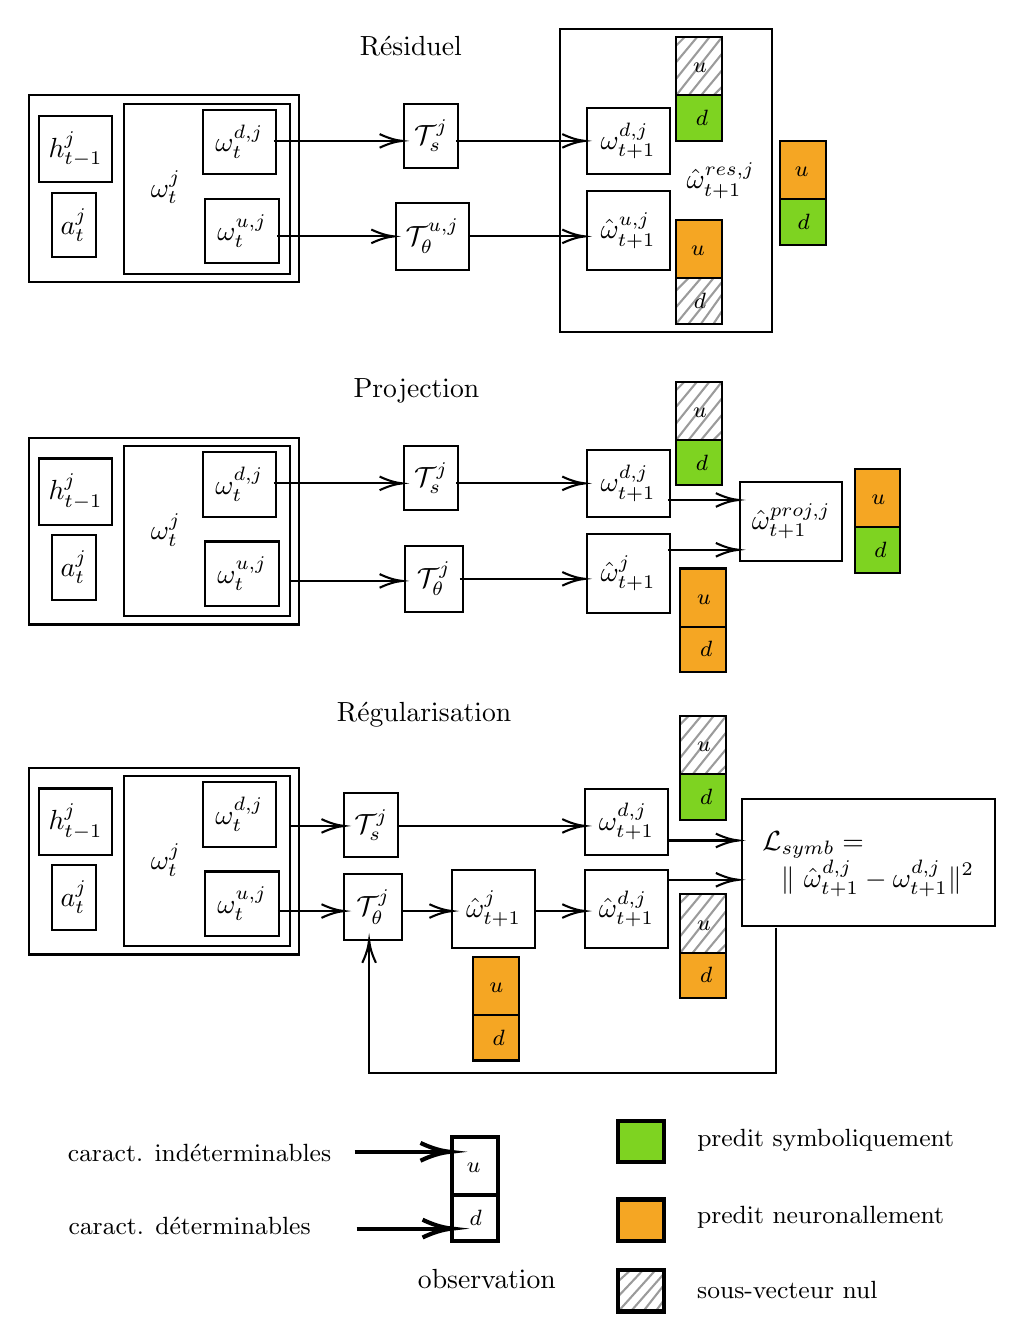
\begin{tikzpicture}[x=0.75pt,y=0.75pt,yscale=-1,xscale=1]
    %uncomment if require: \path (0,5232); %set diagram left start at 0, and has height of 5232

    %Straight Lines [id:da24763982027429865] 
    \draw [color={rgb, 255:red, 155; green, 155; blue, 155 }  ,draw opacity=1 ][fill={rgb, 255:red, 128; green, 128; blue, 128 }  ,fill opacity=1 ][line width=0.75]    (402,4448) -- (384,4470) ;
    %Straight Lines [id:da19980478632170595] 
    \draw [color={rgb, 255:red, 155; green, 155; blue, 155 }  ,draw opacity=1 ][fill={rgb, 255:red, 128; green, 128; blue, 128 }  ,fill opacity=1 ][line width=0.75]    (396,4448) -- (384,4462) ;
    %Straight Lines [id:da32412855340391855] 
    \draw [color={rgb, 255:red, 155; green, 155; blue, 155 }  ,draw opacity=1 ][fill={rgb, 255:red, 128; green, 128; blue, 128 }  ,fill opacity=1 ][line width=0.75]    (406,4450) -- (390,4470) ;
    %Straight Lines [id:da21125524013600872] 
    \draw [color={rgb, 255:red, 155; green, 155; blue, 155 }  ,draw opacity=1 ][fill={rgb, 255:red, 128; green, 128; blue, 128 }  ,fill opacity=1 ][line width=0.75]    (406,4456) -- (396,4470) ;
    %Straight Lines [id:da8737340062156574] 
    \draw [color={rgb, 255:red, 155; green, 155; blue, 155 }  ,draw opacity=1 ][fill={rgb, 255:red, 128; green, 128; blue, 128 }  ,fill opacity=1 ][line width=0.75]    (406,4464) -- (402,4470) ;
    %Straight Lines [id:da2890333682601931] 
    \draw [color={rgb, 255:red, 155; green, 155; blue, 155 }  ,draw opacity=1 ][fill={rgb, 255:red, 128; green, 128; blue, 128 }  ,fill opacity=1 ][line width=0.75]    (384,4454) -- (390,4448) ;
    %Straight Lines [id:da4621444959459615] 
    \draw [color={rgb, 255:red, 155; green, 155; blue, 155 }  ,draw opacity=1 ][fill={rgb, 255:red, 128; green, 128; blue, 128 }  ,fill opacity=1 ][line width=0.75]    (406,4332) -- (384,4360) ;
    %Straight Lines [id:da5637690900595229] 
    \draw [color={rgb, 255:red, 155; green, 155; blue, 155 }  ,draw opacity=1 ][fill={rgb, 255:red, 128; green, 128; blue, 128 }  ,fill opacity=1 ][line width=0.75]    (400,4332) -- (384,4352) ;
    %Straight Lines [id:da7986277651239229] 
    \draw [color={rgb, 255:red, 155; green, 155; blue, 155 }  ,draw opacity=1 ][fill={rgb, 255:red, 128; green, 128; blue, 128 }  ,fill opacity=1 ][line width=0.75]    (406,4340) -- (390,4360) ;
    %Straight Lines [id:da2888528174156788] 
    \draw [color={rgb, 255:red, 155; green, 155; blue, 155 }  ,draw opacity=1 ][fill={rgb, 255:red, 128; green, 128; blue, 128 }  ,fill opacity=1 ][line width=0.75]    (406,4348) -- (396,4360) ;
    %Straight Lines [id:da21145998471436278] 
    \draw [color={rgb, 255:red, 155; green, 155; blue, 155 }  ,draw opacity=1 ][fill={rgb, 255:red, 128; green, 128; blue, 128 }  ,fill opacity=1 ][line width=0.75]    (406,4356) -- (402,4360) ;
    %Straight Lines [id:da259794037058905] 
    \draw [color={rgb, 255:red, 155; green, 155; blue, 155 }  ,draw opacity=1 ][fill={rgb, 255:red, 128; green, 128; blue, 128 }  ,fill opacity=1 ][line width=0.75]    (384,4344) -- (394,4332) ;
    %Straight Lines [id:da37905992722226245] 
    \draw [color={rgb, 255:red, 155; green, 155; blue, 155 }  ,draw opacity=1 ][fill={rgb, 255:red, 128; green, 128; blue, 128 }  ,fill opacity=1 ][line width=0.75]    (384,4336) -- (388,4332) ;

    %Straight Lines [id:da4618897886186095] 
    \draw [color={rgb, 255:red, 155; green, 155; blue, 155 }  ,draw opacity=1 ][fill={rgb, 255:red, 128; green, 128; blue, 128 }  ,fill opacity=1 ][line width=0.75]    (406,4498) -- (384,4526) ;
    %Straight Lines [id:da9618492285817379] 
    \draw [color={rgb, 255:red, 155; green, 155; blue, 155 }  ,draw opacity=1 ][fill={rgb, 255:red, 128; green, 128; blue, 128 }  ,fill opacity=1 ][line width=0.75]    (400,4498) -- (384,4518) ;
    %Straight Lines [id:da4047027863035557] 
    \draw [color={rgb, 255:red, 155; green, 155; blue, 155 }  ,draw opacity=1 ][fill={rgb, 255:red, 128; green, 128; blue, 128 }  ,fill opacity=1 ][line width=0.75]    (406,4506) -- (390,4526) ;
    %Straight Lines [id:da2338233317691657] 
    \draw [color={rgb, 255:red, 155; green, 155; blue, 155 }  ,draw opacity=1 ][fill={rgb, 255:red, 128; green, 128; blue, 128 }  ,fill opacity=1 ][line width=0.75]    (406,4514) -- (396,4526) ;
    %Straight Lines [id:da040061497129813106] 
    \draw [color={rgb, 255:red, 155; green, 155; blue, 155 }  ,draw opacity=1 ][fill={rgb, 255:red, 128; green, 128; blue, 128 }  ,fill opacity=1 ][line width=0.75]    (406,4522) -- (402,4526) ;
    %Straight Lines [id:da8926300803967907] 
    \draw [color={rgb, 255:red, 155; green, 155; blue, 155 }  ,draw opacity=1 ][fill={rgb, 255:red, 128; green, 128; blue, 128 }  ,fill opacity=1 ][line width=0.75]    (384,4510) -- (394,4498) ;
    %Straight Lines [id:da8033717813225199] 
    \draw [color={rgb, 255:red, 155; green, 155; blue, 155 }  ,draw opacity=1 ][fill={rgb, 255:red, 128; green, 128; blue, 128 }  ,fill opacity=1 ][line width=0.75]    (384,4502) -- (388,4498) ;

    %Straight Lines [id:da7989858669141804] 
    \draw [color={rgb, 255:red, 155; green, 155; blue, 155 }  ,draw opacity=1 ][fill={rgb, 255:red, 128; green, 128; blue, 128 }  ,fill opacity=1 ][line width=0.75]    (408,4659.05) -- (386,4687.05) ;
    %Straight Lines [id:da40202240481802576] 
    \draw [color={rgb, 255:red, 155; green, 155; blue, 155 }  ,draw opacity=1 ][fill={rgb, 255:red, 128; green, 128; blue, 128 }  ,fill opacity=1 ][line width=0.75]    (402,4659.05) -- (386,4679.05) ;
    %Straight Lines [id:da23397697614023283] 
    \draw [color={rgb, 255:red, 155; green, 155; blue, 155 }  ,draw opacity=1 ][fill={rgb, 255:red, 128; green, 128; blue, 128 }  ,fill opacity=1 ][line width=0.75]    (408,4667.05) -- (392,4687.05) ;
    %Straight Lines [id:da5091139872418293] 
    \draw [color={rgb, 255:red, 155; green, 155; blue, 155 }  ,draw opacity=1 ][fill={rgb, 255:red, 128; green, 128; blue, 128 }  ,fill opacity=1 ][line width=0.75]    (408,4675.05) -- (398,4687.05) ;
    %Straight Lines [id:da7838519186238893] 
    \draw [color={rgb, 255:red, 155; green, 155; blue, 155 }  ,draw opacity=1 ][fill={rgb, 255:red, 128; green, 128; blue, 128 }  ,fill opacity=1 ][line width=0.75]    (408,4683.05) -- (404,4687.05) ;
    %Straight Lines [id:da15998290322205744] 
    \draw [color={rgb, 255:red, 155; green, 155; blue, 155 }  ,draw opacity=1 ][fill={rgb, 255:red, 128; green, 128; blue, 128 }  ,fill opacity=1 ][line width=0.75]    (386,4671.05) -- (396,4659.05) ;
    %Straight Lines [id:da2930214299406628] 
    \draw [color={rgb, 255:red, 155; green, 155; blue, 155 }  ,draw opacity=1 ][fill={rgb, 255:red, 128; green, 128; blue, 128 }  ,fill opacity=1 ][line width=0.75]    (386,4663.05) -- (390,4659.05) ;

    %Straight Lines [id:da560381072959208] 
    \draw [color={rgb, 255:red, 155; green, 155; blue, 155 }  ,draw opacity=1 ][fill={rgb, 255:red, 128; green, 128; blue, 128 }  ,fill opacity=1 ][line width=0.75]    (408,4745.05) -- (386,4773.05) ;
    %Straight Lines [id:da019087143657265826] 
    \draw [color={rgb, 255:red, 155; green, 155; blue, 155 }  ,draw opacity=1 ][fill={rgb, 255:red, 128; green, 128; blue, 128 }  ,fill opacity=1 ][line width=0.75]    (402,4745.05) -- (386,4765.05) ;
    %Straight Lines [id:da1302277202981762] 
    \draw [color={rgb, 255:red, 155; green, 155; blue, 155 }  ,draw opacity=1 ][fill={rgb, 255:red, 128; green, 128; blue, 128 }  ,fill opacity=1 ][line width=0.75]    (408,4753.05) -- (392,4773.05) ;
    %Straight Lines [id:da09652292926698536] 
    \draw [color={rgb, 255:red, 155; green, 155; blue, 155 }  ,draw opacity=1 ][fill={rgb, 255:red, 128; green, 128; blue, 128 }  ,fill opacity=1 ][line width=0.75]    (408,4761.05) -- (398,4773.05) ;
    %Straight Lines [id:da7503736353080281] 
    \draw [color={rgb, 255:red, 155; green, 155; blue, 155 }  ,draw opacity=1 ][fill={rgb, 255:red, 128; green, 128; blue, 128 }  ,fill opacity=1 ][line width=0.75]    (408,4769.05) -- (404,4773.05) ;
    %Straight Lines [id:da5657791005138578] 
    \draw [color={rgb, 255:red, 155; green, 155; blue, 155 }  ,draw opacity=1 ][fill={rgb, 255:red, 128; green, 128; blue, 128 }  ,fill opacity=1 ][line width=0.75]    (386,4757.05) -- (396,4745.05) ;
    %Straight Lines [id:da24043326957092126] 
    \draw [color={rgb, 255:red, 155; green, 155; blue, 155 }  ,draw opacity=1 ][fill={rgb, 255:red, 128; green, 128; blue, 128 }  ,fill opacity=1 ][line width=0.75]    (386,4749.05) -- (390,4745.05) ;

    %Shape: Rectangle [id:dp9707159588190506] 
    \draw   (72,4360) -- (202,4360) -- (202,4450) -- (72,4450) -- cycle ;
    %Shape: Rectangle [id:dp5706382238892072] 
    \draw   (328,4328) -- (430,4328) -- (430,4474) -- (328,4474) -- cycle ;
    %Straight Lines [id:da7375663634648962] 
    \draw    (190,4382) -- (250,4382) ;
    \draw [shift={(252,4382)}, rotate = 180] [color={rgb, 255:red, 0; green, 0; blue, 0 }  ][line width=0.75]    (10.93,-3.29) .. controls (6.95,-1.4) and (3.31,-0.3) .. (0,0) .. controls (3.31,0.3) and (6.95,1.4) .. (10.93,3.29)   ;
    %Straight Lines [id:da1312146218906476] 
    \draw    (191.68,4428) -- (246,4428) ;
    \draw [shift={(248,4428)}, rotate = 180] [color={rgb, 255:red, 0; green, 0; blue, 0 }  ][line width=0.75]    (10.93,-3.29) .. controls (6.95,-1.4) and (3.31,-0.3) .. (0,0) .. controls (3.31,0.3) and (6.95,1.4) .. (10.93,3.29)   ;
    %Straight Lines [id:da20293234879784128] 
    \draw    (278,4382) -- (338,4382) ;
    \draw [shift={(340,4382)}, rotate = 180] [color={rgb, 255:red, 0; green, 0; blue, 0 }  ][line width=0.75]    (10.93,-3.29) .. controls (6.95,-1.4) and (3.31,-0.3) .. (0,0) .. controls (3.31,0.3) and (6.95,1.4) .. (10.93,3.29)   ;
    %Straight Lines [id:da7780554830331595] 
    \draw    (284,4428) -- (338,4428) ;
    \draw [shift={(340,4428)}, rotate = 180] [color={rgb, 255:red, 0; green, 0; blue, 0 }  ][line width=0.75]    (10.93,-3.29) .. controls (6.95,-1.4) and (3.31,-0.3) .. (0,0) .. controls (3.31,0.3) and (6.95,1.4) .. (10.93,3.29)   ;
    %Shape: Rectangle [id:dp9989891710916556] 
    \draw   (118,4364) -- (198,4364) -- (198,4446) -- (118,4446) -- cycle ;
    %Shape: Rectangle [id:dp5273520585937012] 
    \draw   (72,4684) -- (202,4684) -- (202,4774) -- (72,4774) -- cycle ;
    %Straight Lines [id:da11653013315343552] 
    \draw    (192,4753.05) -- (222,4753.05) ;
    \draw [shift={(224,4753.05)}, rotate = 180] [color={rgb, 255:red, 0; green, 0; blue, 0 }  ][line width=0.75]    (10.93,-3.29) .. controls (6.95,-1.4) and (3.31,-0.3) .. (0,0) .. controls (3.31,0.3) and (6.95,1.4) .. (10.93,3.29)   ;
    %Straight Lines [id:da2685409551114073] 
    \draw    (250,4712.05) -- (338,4712.05) ;
    \draw [shift={(340,4712.05)}, rotate = 180] [color={rgb, 255:red, 0; green, 0; blue, 0 }  ][line width=0.75]    (10.93,-3.29) .. controls (6.95,-1.4) and (3.31,-0.3) .. (0,0) .. controls (3.31,0.3) and (6.95,1.4) .. (10.93,3.29)   ;
    %Straight Lines [id:da6588342775342261] 
    \draw    (316,4753.05) -- (333.67,4753.05) -- (338,4753.05) ;
    \draw [shift={(340,4753.05)}, rotate = 180] [color={rgb, 255:red, 0; green, 0; blue, 0 }  ][line width=0.75]    (10.93,-3.29) .. controls (6.95,-1.4) and (3.31,-0.3) .. (0,0) .. controls (3.31,0.3) and (6.95,1.4) .. (10.93,3.29)   ;
    %Shape: Rectangle [id:dp9055792744513167] 
    \draw   (118,4688) -- (198,4688) -- (198,4770) -- (118,4770) -- cycle ;
    %Straight Lines [id:da005030131609338517] 
    \draw    (432,4761.05) -- (432,4831.05) -- (236,4831.05) -- (236,4769.05) ;
    \draw [shift={(236,4767.05)}, rotate = 90] [color={rgb, 255:red, 0; green, 0; blue, 0 }  ][line width=0.75]    (10.93,-3.29) .. controls (6.95,-1.4) and (3.31,-0.3) .. (0,0) .. controls (3.31,0.3) and (6.95,1.4) .. (10.93,3.29)   ;
    %Straight Lines [id:da24266384766556137] 
    \draw    (380,4719.05) -- (412,4719.05) ;
    \draw [shift={(414,4719.05)}, rotate = 180] [color={rgb, 255:red, 0; green, 0; blue, 0 }  ][line width=0.75]    (10.93,-3.29) .. controls (6.95,-1.4) and (3.31,-0.3) .. (0,0) .. controls (3.31,0.3) and (6.95,1.4) .. (10.93,3.29)   ;
    %Straight Lines [id:da7310522190261277] 
    \draw    (380,4738) -- (412,4738) ;
    \draw [shift={(414,4738)}, rotate = 180] [color={rgb, 255:red, 0; green, 0; blue, 0 }  ][line width=0.75]    (10.93,-3.29) .. controls (6.95,-1.4) and (3.31,-0.3) .. (0,0) .. controls (3.31,0.3) and (6.95,1.4) .. (10.93,3.29)   ;
    %Shape: Rectangle [id:dp7311570933646381] 
    \draw   (72,4525) -- (202,4525) -- (202,4615) -- (72,4615) -- cycle ;
    %Straight Lines [id:da3798900997456174] 
    \draw    (190,4547) -- (250,4547) ;
    \draw [shift={(252,4547)}, rotate = 180] [color={rgb, 255:red, 0; green, 0; blue, 0 }  ][line width=0.75]    (10.93,-3.29) .. controls (6.95,-1.4) and (3.31,-0.3) .. (0,0) .. controls (3.31,0.3) and (6.95,1.4) .. (10.93,3.29)   ;
    %Straight Lines [id:da2994143489873299] 
    \draw    (198,4594) -- (250,4594) ;
    \draw [shift={(252,4594)}, rotate = 180] [color={rgb, 255:red, 0; green, 0; blue, 0 }  ][line width=0.75]    (10.93,-3.29) .. controls (6.95,-1.4) and (3.31,-0.3) .. (0,0) .. controls (3.31,0.3) and (6.95,1.4) .. (10.93,3.29)   ;
    %Straight Lines [id:da5138987789523812] 
    \draw    (278,4547) -- (338,4547) ;
    \draw [shift={(340,4547)}, rotate = 180] [color={rgb, 255:red, 0; green, 0; blue, 0 }  ][line width=0.75]    (10.93,-3.29) .. controls (6.95,-1.4) and (3.31,-0.3) .. (0,0) .. controls (3.31,0.3) and (6.95,1.4) .. (10.93,3.29)   ;
    %Straight Lines [id:da008609447431192963] 
    \draw    (279.68,4593) -- (338,4593) ;
    \draw [shift={(340,4593)}, rotate = 180] [color={rgb, 255:red, 0; green, 0; blue, 0 }  ][line width=0.75]    (10.93,-3.29) .. controls (6.95,-1.4) and (3.31,-0.3) .. (0,0) .. controls (3.31,0.3) and (6.95,1.4) .. (10.93,3.29)   ;
    %Shape: Rectangle [id:dp6195597507073775] 
    \draw   (118,4529) -- (198,4529) -- (198,4611) -- (118,4611) -- cycle ;
    %Straight Lines [id:da7573621456959849] 
    \draw    (380,4555) -- (412,4555) ;
    \draw [shift={(414,4555)}, rotate = 180] [color={rgb, 255:red, 0; green, 0; blue, 0 }  ][line width=0.75]    (10.93,-3.29) .. controls (6.95,-1.4) and (3.31,-0.3) .. (0,0) .. controls (3.31,0.3) and (6.95,1.4) .. (10.93,3.29)   ;
    %Straight Lines [id:da4158752259413163] 
    \draw    (380,4579) -- (412,4579) ;
    \draw [shift={(414,4579)}, rotate = 180] [color={rgb, 255:red, 0; green, 0; blue, 0 }  ][line width=0.75]    (10.93,-3.29) .. controls (6.95,-1.4) and (3.31,-0.3) .. (0,0) .. controls (3.31,0.3) and (6.95,1.4) .. (10.93,3.29)   ;
    %Straight Lines [id:da9101547299454278] 
    \draw    (198,4712.05) -- (211,4712.05) -- (222,4712.05) ;
    \draw [shift={(224,4712.05)}, rotate = 180] [color={rgb, 255:red, 0; green, 0; blue, 0 }  ][line width=0.75]    (10.93,-3.29) .. controls (6.95,-1.4) and (3.31,-0.3) .. (0,0) .. controls (3.31,0.3) and (6.95,1.4) .. (10.93,3.29)   ;
    %Shape: Rectangle [id:dp5266308820425851] 
    \draw   (384,4498) -- (406,4498) -- (406,4548) -- (384,4548) -- cycle ;
    %Shape: Rectangle [id:dp4591330400004242] 
    \draw  [color={rgb, 255:red, 0; green, 0; blue, 0 }  ,draw opacity=1 ][fill={rgb, 255:red, 126; green, 211; blue, 33 }  ,fill opacity=1 ] (384,4526) -- (406,4526) -- (406,4548) -- (384,4548) -- cycle ;
    %Shape: Rectangle [id:dp361348098683958] 
    \draw  [color={rgb, 255:red, 0; green, 0; blue, 0 }  ,draw opacity=1 ][fill={rgb, 255:red, 245; green, 166; blue, 35 }  ,fill opacity=1 ][line width=1.5]  (355.97,4892.05) -- (377.97,4892.05) -- (377.97,4912.05) -- (355.97,4912.05) -- cycle ;
    %Shape: Rectangle [id:dp9964835829419468] 
    \draw  [color={rgb, 255:red, 0; green, 0; blue, 0 }  ,draw opacity=1 ][fill={rgb, 255:red, 126; green, 211; blue, 33 }  ,fill opacity=1 ][line width=1.5]  (355.97,4854.05) -- (377.97,4854.05) -- (377.97,4874.05) -- (355.97,4874.05) -- cycle ;
    %Shape: Rectangle [id:dp33016566097204514] 
    \draw  [line width=1.5]  (275.97,4862.05) -- (297.97,4862.05) -- (297.97,4912.05) -- (275.97,4912.05) -- cycle ;
    %Shape: Rectangle [id:dp5620232952994356] 
    \draw  [color={rgb, 255:red, 0; green, 0; blue, 0 }  ,draw opacity=1 ][line width=1.5]  (275.97,4890.05) -- (297.97,4890.05) -- (297.97,4912.05) -- (275.97,4912.05) -- cycle ;
    %Straight Lines [id:da06282474626147139] 
    \draw [line width=1.5]    (229.97,4906.05) -- (272.97,4906.05) ;
    \draw [shift={(275.97,4906.05)}, rotate = 180] [color={rgb, 255:red, 0; green, 0; blue, 0 }  ][line width=1.5]    (14.21,-4.28) .. controls (9.04,-1.82) and (4.3,-0.39) .. (0,0) .. controls (4.3,0.39) and (9.04,1.82) .. (14.21,4.28)   ;
    %Straight Lines [id:da6635137750841066] 
    \draw [line width=1.5]    (228.97,4869.05) -- (271.97,4869.05) ;
    \draw [shift={(274.97,4869.05)}, rotate = 180] [color={rgb, 255:red, 0; green, 0; blue, 0 }  ][line width=1.5]    (14.21,-4.28) .. controls (9.04,-1.82) and (4.3,-0.39) .. (0,0) .. controls (4.3,0.39) and (9.04,1.82) .. (14.21,4.28)   ;
    %Shape: Rectangle [id:dp1847356006106129] 
    \draw  [fill={rgb, 255:red, 245; green, 166; blue, 35 }  ,fill opacity=1 ] (386,4588) -- (408,4588) -- (408,4638) -- (386,4638) -- cycle ;
    %Shape: Rectangle [id:dp25889441177392947] 
    \draw  [color={rgb, 255:red, 0; green, 0; blue, 0 }  ,draw opacity=1 ][fill={rgb, 255:red, 245; green, 166; blue, 35 }  ,fill opacity=1 ] (386,4616) -- (408,4616) -- (408,4638) -- (386,4638) -- cycle ;
    %Shape: Rectangle [id:dp5475751790971162] 
    \draw  [fill={rgb, 255:red, 245; green, 166; blue, 35 }  ,fill opacity=1 ] (470,4540) -- (492,4540) -- (492,4590) -- (470,4590) -- cycle ;
    %Shape: Rectangle [id:dp13145099987658582] 
    \draw  [color={rgb, 255:red, 0; green, 0; blue, 0 }  ,draw opacity=1 ][fill={rgb, 255:red, 126; green, 211; blue, 33 }  ,fill opacity=1 ] (470,4568) -- (492,4568) -- (492,4590) -- (470,4590) -- cycle ;
    %Shape: Rectangle [id:dp5607039901394576] 
    \draw   (384,4332) -- (406,4332) -- (406,4382) -- (384,4382) -- cycle ;
    %Shape: Rectangle [id:dp7284235146248617] 
    \draw  [color={rgb, 255:red, 0; green, 0; blue, 0 }  ,draw opacity=1 ][fill={rgb, 255:red, 126; green, 211; blue, 33 }  ,fill opacity=1 ] (384,4360) -- (406,4360) -- (406,4382) -- (384,4382) -- cycle ;
    %Shape: Rectangle [id:dp011144053288704048] 
    \draw  [fill={rgb, 255:red, 245; green, 166; blue, 35 }  ,fill opacity=1 ] (384,4420) -- (406,4420) -- (406,4448) -- (384,4448) -- cycle ;
    %Shape: Rectangle [id:dp8896868698611735] 
    \draw  [color={rgb, 255:red, 0; green, 0; blue, 0 }  ,draw opacity=1 ] (384,4448) -- (406,4448) -- (406,4470) -- (384,4470) -- cycle ;
    %Shape: Rectangle [id:dp44625969909571783] 
    \draw  [fill={rgb, 255:red, 245; green, 166; blue, 35 }  ,fill opacity=1 ] (434,4382) -- (456,4382) -- (456,4432) -- (434,4432) -- cycle ;
    %Shape: Rectangle [id:dp9758623501572419] 
    \draw  [color={rgb, 255:red, 0; green, 0; blue, 0 }  ,draw opacity=1 ][fill={rgb, 255:red, 126; green, 211; blue, 33 }  ,fill opacity=1 ] (434,4410) -- (456,4410) -- (456,4432) -- (434,4432) -- cycle ;
    %Shape: Rectangle [id:dp31106797237154105] 
    \draw   (386,4659.05) -- (408,4659.05) -- (408,4709.05) -- (386,4709.05) -- cycle ;
    %Shape: Rectangle [id:dp37748168173399266] 
    \draw  [color={rgb, 255:red, 0; green, 0; blue, 0 }  ,draw opacity=1 ][fill={rgb, 255:red, 126; green, 211; blue, 33 }  ,fill opacity=1 ] (386,4687.05) -- (408,4687.05) -- (408,4709.05) -- (386,4709.05) -- cycle ;
    %Shape: Rectangle [id:dp36373534246672357] 
    \draw   (386,4745.05) -- (408,4745.05) -- (408,4773.05) -- (386,4773.05) -- cycle ;
    %Shape: Rectangle [id:dp9380907801253754] 
    \draw  [color={rgb, 255:red, 0; green, 0; blue, 0 }  ,draw opacity=1 ][fill={rgb, 255:red, 245; green, 166; blue, 35 }  ,fill opacity=1 ] (386,4773.05) -- (408,4773.05) -- (408,4795.05) -- (386,4795.05) -- cycle ;
    %Straight Lines [id:da9354080425661864] 
    \draw    (252,4753.05) -- (274,4753.05) ;
    \draw [shift={(276,4753.05)}, rotate = 180] [color={rgb, 255:red, 0; green, 0; blue, 0 }  ][line width=0.75]    (10.93,-3.29) .. controls (6.95,-1.4) and (3.31,-0.3) .. (0,0) .. controls (3.31,0.3) and (6.95,1.4) .. (10.93,3.29)   ;
    %Shape: Rectangle [id:dp18329706016338654] 
    \draw  [fill={rgb, 255:red, 245; green, 166; blue, 35 }  ,fill opacity=1 ] (286,4775.05) -- (308,4775.05) -- (308,4825.05) -- (286,4825.05) -- cycle ;
    %Shape: Rectangle [id:dp3467980434275424] 
    \draw  [color={rgb, 255:red, 0; green, 0; blue, 0 }  ,draw opacity=1 ][fill={rgb, 255:red, 245; green, 166; blue, 35 }  ,fill opacity=1 ] (286,4803.05) -- (308,4803.05) -- (308,4825.05) -- (286,4825.05) -- cycle ;
    %Straight Lines [id:da8580945385081316] 
    \draw [color={rgb, 255:red, 155; green, 155; blue, 155 }  ,draw opacity=1 ][fill={rgb, 255:red, 128; green, 128; blue, 128 }  ,fill opacity=1 ][line width=0.75]    (374,4926) -- (356,4946) ;
    %Straight Lines [id:da9112126259690438] 
    \draw [color={rgb, 255:red, 155; green, 155; blue, 155 }  ,draw opacity=1 ][fill={rgb, 255:red, 128; green, 128; blue, 128 }  ,fill opacity=1 ][line width=0.75]    (368,4926) -- (356,4938.73) ;
    %Straight Lines [id:da5513034474442061] 
    \draw [color={rgb, 255:red, 155; green, 155; blue, 155 }  ,draw opacity=1 ][fill={rgb, 255:red, 128; green, 128; blue, 128 }  ,fill opacity=1 ][line width=0.75]    (378,4927.82) -- (362,4946) ;
    %Straight Lines [id:da7585606171855108] 
    \draw [color={rgb, 255:red, 155; green, 155; blue, 155 }  ,draw opacity=1 ][fill={rgb, 255:red, 128; green, 128; blue, 128 }  ,fill opacity=1 ][line width=0.75]    (378,4933.27) -- (368,4946) ;
    %Straight Lines [id:da6936034571787613] 
    \draw [color={rgb, 255:red, 155; green, 155; blue, 155 }  ,draw opacity=1 ][fill={rgb, 255:red, 128; green, 128; blue, 128 }  ,fill opacity=1 ][line width=0.75]    (378,4940.55) -- (374,4946) ;
    %Straight Lines [id:da367549950619389] 
    \draw [color={rgb, 255:red, 155; green, 155; blue, 155 }  ,draw opacity=1 ][fill={rgb, 255:red, 128; green, 128; blue, 128 }  ,fill opacity=1 ][line width=0.75]    (356,4931.45) -- (362,4926) ;
    %Shape: Rectangle [id:dp5855170308849831] 
    \draw  [color={rgb, 255:red, 0; green, 0; blue, 0 }  ,draw opacity=1 ][line width=1.5]  (356,4926) -- (378,4926) -- (378,4946) -- (356,4946) -- cycle ;


    % Text Node
    \draw (437.5,4935.5) node  [font=\small] [align=left] {sous-vecteur nul};
    % Text Node
    \draw (298.38,4814.05) node  [font=\footnotesize] [align=left] {$\displaystyle d$};
    % Text Node
    \draw (297.38,4790.05) node  [font=\footnotesize] [align=left] {$\displaystyle u$};
    % Text Node
    \draw (149.5,4904.55) node  [font=\small] [align=left] {caract. déterminables};
    % Text Node
    \draw (154.26,4869.5) node  [font=\small] [align=left] {caract. indéterminables};
    % Text Node
    \draw (292.75,4930.55) node   [align=left] {observation};
    % Text Node
    \draw (287.34,4900.95) node  [font=\footnotesize] [align=left] {$\displaystyle d$};
    % Text Node
    \draw (286.34,4876.95) node  [font=\footnotesize] [align=left] {$\displaystyle u$};
    % Text Node
    \draw (453.5,4900.55) node  [font=\small] [align=left] {predit neuronallement};
    % Text Node
    \draw (456,4863.5) node  [font=\small] [align=left] {predit symboliquement};
    % Text Node
    \draw    (276,4733.05) -- (316,4733.05) -- (316,4771.05) -- (276,4771.05) -- cycle  ;
    \draw (296,4752.05) node   [align=left] {$\displaystyle \hat{\omega }_{t+1}^{j}$};
    % Text Node
    \draw (398.38,4784.05) node  [font=\footnotesize] [align=left] {$\displaystyle d$};
    % Text Node
    \draw (397.38,4760.05) node  [font=\footnotesize] [align=left] {$\displaystyle u$};
    % Text Node
    \draw (398.38,4698.05) node  [font=\footnotesize] [align=left] {$\displaystyle d$};
    % Text Node
    \draw (397.38,4674.05) node  [font=\footnotesize] [align=left] {$\displaystyle u$};
    % Text Node
    \draw (445.38,4420.9) node  [font=\footnotesize] [align=left] {$\displaystyle d$};
    % Text Node
    \draw (444.38,4396.9) node  [font=\footnotesize] [align=left] {$\displaystyle u$};
    % Text Node
    \draw (395.38,4458.9) node  [font=\footnotesize] [align=left] {$\displaystyle d$};
    % Text Node
    \draw (394.38,4434.9) node  [font=\footnotesize] [align=left] {$\displaystyle u$};
    % Text Node
    \draw (396.38,4371) node  [font=\footnotesize] [align=left] {$\displaystyle d$};
    % Text Node
    \draw (395.38,4347) node  [font=\footnotesize] [align=left] {$\displaystyle u$};
    % Text Node
    \draw (482.38,4579) node  [font=\footnotesize] [align=left] {$\displaystyle d$};
    % Text Node
    \draw (481.38,4555) node  [font=\footnotesize] [align=left] {$\displaystyle u$};
    % Text Node
    \draw (398.38,4627) node  [font=\footnotesize] [align=left] {$\displaystyle d$};
    % Text Node
    \draw (397.38,4603) node  [font=\footnotesize] [align=left] {$\displaystyle u$};
    % Text Node
    \draw (396.38,4537) node  [font=\footnotesize] [align=left] {$\displaystyle d$};
    % Text Node
    \draw (395.38,4513) node  [font=\footnotesize] [align=left] {$\displaystyle u$};
    % Text Node
    \draw    (414.86,4546.34) -- (463.86,4546.34) -- (463.86,4584.34) -- (414.86,4584.34) -- cycle  ;
    \draw (439.36,4565.34) node   [align=left] {$\displaystyle \hat{\omega }_{t+1}^{proj,j}$};
    % Text Node
    \draw (227,4495) node [anchor=north west][inner sep=0.75pt]   [align=left] {Projection};
    % Text Node
    \draw    (340.76,4571.34) -- (380.76,4571.34) -- (380.76,4609.34) -- (340.76,4609.34) -- cycle  ;
    \draw (360.76,4590.34) node   [align=left] {$\displaystyle \hat{\omega }_{t+1}^{j}$};
    % Text Node
    \draw    (340.76,4531) -- (380.76,4531) -- (380.76,4563) -- (340.76,4563) -- cycle  ;
    \draw (360.76,4547) node   [align=left] {$\displaystyle \omega _{t+1}^{d,j}$};
    % Text Node
    \draw    (253.2,4577) -- (281.2,4577) -- (281.2,4609) -- (253.2,4609) -- cycle  ;
    \draw (267.2,4593) node   [align=left] {$\displaystyle \mathcal{T}_{\theta }^{j}$};
    % Text Node
    \draw    (252.86,4529) -- (278.86,4529) -- (278.86,4560) -- (252.86,4560) -- cycle  ;
    \draw (265.86,4544.5) node   [align=left] {$\displaystyle \mathcal{T}_{s}^{j}$};
    % Text Node
    \draw    (156.8,4575) -- (192.8,4575) -- (192.8,4606) -- (156.8,4606) -- cycle  ;
    \draw (174.8,4590.5) node   [align=left] {$\displaystyle \omega _{t}^{u,j}$};
    % Text Node
    \draw    (155.98,4532) -- (190.98,4532) -- (190.98,4563) -- (155.98,4563) -- cycle  ;
    \draw (173.48,4547.5) node   [align=left] {$\displaystyle \omega _{t}^{d,j}$};
    % Text Node
    \draw (138.02,4569.5) node   [align=left] {$\displaystyle \omega _{t}^{j}$};
    % Text Node
    \draw    (83.21,4572) -- (104.21,4572) -- (104.21,4603) -- (83.21,4603) -- cycle  ;
    \draw (93.71,4587.5) node   [align=left] {$\displaystyle a_{t}^{j}$};
    % Text Node
    \draw    (77.05,4535) -- (112.05,4535) -- (112.05,4567) -- (77.05,4567) -- cycle  ;
    \draw (94.55,4551) node   [align=left] {$\displaystyle h_{t-1}^{j}$};
    % Text Node
    \draw    (415.5,4699.03) -- (537.5,4699.03) -- (537.5,4760.03) -- (415.5,4760.03) -- cycle  ;
    \draw (476.5,4729.53) node   [align=left] {$\displaystyle  \begin{array}{{>{\displaystyle}l}}
                \mathcal{L}_{symb} = \\
                \ \ \| \ \hat{\omega }_{t+1}^{d,j} -\omega _{t+1}^{d,j} \| ^{2}
            \end{array}$};
    % Text Node
    \draw (219,4651) node [anchor=north west][inner sep=0.75pt]   [align=left] {Régularisation};
    % Text Node
    \draw    (340,4733.05) -- (380,4733.05) -- (380,4771.05) -- (340,4771.05) -- cycle  ;
    \draw (360,4752.05) node   [align=left] {$\displaystyle \hat{\omega }_{t+1}^{d,j}$};
    % Text Node
    \draw    (340,4694.05) -- (380,4694.05) -- (380,4726.05) -- (340,4726.05) -- cycle  ;
    \draw (360,4710.05) node   [align=left] {$\displaystyle \omega _{t+1}^{d,j}$};
    % Text Node
    \draw    (224,4735.05) -- (252,4735.05) -- (252,4767.05) -- (224,4767.05) -- cycle  ;
    \draw (238,4751.05) node   [align=left] {$\displaystyle \mathcal{T}_{\theta }^{j}$};
    % Text Node
    \draw    (224.01,4696.05) -- (250.01,4696.05) -- (250.01,4727.05) -- (224.01,4727.05) -- cycle  ;
    \draw (237.01,4711.55) node   [align=left] {$\displaystyle \mathcal{T}_{s}^{j}$};
    % Text Node
    \draw    (156.8,4734) -- (192.8,4734) -- (192.8,4765) -- (156.8,4765) -- cycle  ;
    \draw (174.8,4749.5) node   [align=left] {$\displaystyle \omega _{t}^{u,j}$};
    % Text Node
    \draw    (155.98,4691) -- (190.98,4691) -- (190.98,4722) -- (155.98,4722) -- cycle  ;
    \draw (173.48,4706.5) node   [align=left] {$\displaystyle \omega _{t}^{d,j}$};
    % Text Node
    \draw (138.02,4728.5) node   [align=left] {$\displaystyle \omega _{t}^{j}$};
    % Text Node
    \draw    (83.21,4731) -- (104.21,4731) -- (104.21,4762) -- (83.21,4762) -- cycle  ;
    \draw (93.71,4746.5) node   [align=left] {$\displaystyle a_{t}^{j}$};
    % Text Node
    \draw    (77.05,4694) -- (112.05,4694) -- (112.05,4726) -- (77.05,4726) -- cycle  ;
    \draw (94.55,4710) node   [align=left] {$\displaystyle h_{t-1}^{j}$};
    % Text Node
    \draw (230,4330) node [anchor=north west][inner sep=0.75pt]   [align=left] {Résiduel};
    % Text Node
    \draw    (340.76,4406.34) -- (380.76,4406.34) -- (380.76,4444.34) -- (340.76,4444.34) -- cycle  ;
    \draw (360.76,4425.34) node   [align=left] {$\displaystyle \hat{\omega }_{t+1}^{u,j}$};
    % Text Node
    \draw    (340.76,4366) -- (380.76,4366) -- (380.76,4398) -- (340.76,4398) -- cycle  ;
    \draw (360.76,4382) node   [align=left] {$\displaystyle \omega _{t+1}^{d,j}$};
    % Text Node
    \draw (405.42,4401.23) node   [align=left] {$\displaystyle \hat{\omega }_{t+1}^{res,j}$};
    % Text Node
    \draw    (249.01,4412) -- (284.01,4412) -- (284.01,4444) -- (249.01,4444) -- cycle  ;
    \draw (266.51,4428) node   [align=left] {$\displaystyle \mathcal{T}_{\theta }^{u,j}$};
    % Text Node
    \draw    (252.86,4364) -- (278.86,4364) -- (278.86,4395) -- (252.86,4395) -- cycle  ;
    \draw (265.86,4379.5) node   [align=left] {$\displaystyle \mathcal{T}_{s}^{j}$};
    % Text Node
    \draw    (156.8,4410) -- (192.8,4410) -- (192.8,4441) -- (156.8,4441) -- cycle  ;
    \draw (174.8,4425.5) node   [align=left] {$\displaystyle \omega _{t}^{u,j}$};
    % Text Node
    \draw    (155.98,4367) -- (190.98,4367) -- (190.98,4398) -- (155.98,4398) -- cycle  ;
    \draw (173.48,4382.5) node   [align=left] {$\displaystyle \omega _{t}^{d,j}$};
    % Text Node
    \draw (138.02,4404.5) node   [align=left] {$\displaystyle \omega _{t}^{j}$};
    % Text Node
    \draw    (83.21,4407) -- (104.21,4407) -- (104.21,4438) -- (83.21,4438) -- cycle  ;
    \draw (93.71,4422.5) node   [align=left] {$\displaystyle a_{t}^{j}$};
    % Text Node
    \draw    (77.05,4370) -- (112.05,4370) -- (112.05,4402) -- (77.05,4402) -- cycle  ;
    \draw (94.55,4386) node   [align=left] {$\displaystyle h_{t-1}^{j}$};


\end{tikzpicture}